\documentclass[12pt,]{article}
\usepackage{lmodern}
\usepackage{amssymb,amsmath}
\usepackage{ifxetex,ifluatex}
\usepackage{fixltx2e} % provides \textsubscript
\ifnum 0\ifxetex 1\fi\ifluatex 1\fi=0 % if pdftex
  \usepackage[T1]{fontenc}
  \usepackage[utf8]{inputenc}
\else % if luatex or xelatex
  \ifxetex
    \usepackage{mathspec}
  \else
    \usepackage{fontspec}
  \fi
  \defaultfontfeatures{Ligatures=TeX,Scale=MatchLowercase}
  \newcommand{\euro}{€}
\fi
% use upquote if available, for straight quotes in verbatim environments
\IfFileExists{upquote.sty}{\usepackage{upquote}}{}
% use microtype if available
\IfFileExists{microtype.sty}{%
\usepackage{microtype}
\UseMicrotypeSet[protrusion]{basicmath} % disable protrusion for tt fonts
}{}
\usepackage[margin=1in]{geometry}
\usepackage{hyperref}
\PassOptionsToPackage{usenames,dvipsnames}{color} % color is loaded by hyperref
\hypersetup{unicode=true,
            pdftitle={Workshop Examples},
            pdfauthor={Melissa Monk},
            pdfborder={0 0 0},
            breaklinks=true}
\urlstyle{same}  % don't use monospace font for urls
\usepackage{graphicx,grffile}
\makeatletter
\def\maxwidth{\ifdim\Gin@nat@width>\linewidth\linewidth\else\Gin@nat@width\fi}
\def\maxheight{\ifdim\Gin@nat@height>\textheight\textheight\else\Gin@nat@height\fi}
\makeatother
% Scale images if necessary, so that they will not overflow the page
% margins by default, and it is still possible to overwrite the defaults
% using explicit options in \includegraphics[width, height, ...]{}
\setkeys{Gin}{width=\maxwidth,height=\maxheight,keepaspectratio}
\setlength{\parindent}{0pt}
\setlength{\parskip}{6pt plus 2pt minus 1pt}
\setlength{\emergencystretch}{3em}  % prevent overfull lines
\providecommand{\tightlist}{%
  \setlength{\itemsep}{0pt}\setlength{\parskip}{0pt}}
\setcounter{secnumdepth}{5}

%%% Use protect on footnotes to avoid problems with footnotes in titles
\let\rmarkdownfootnote\footnote%
\def\footnote{\protect\rmarkdownfootnote}

%%% Change title format to be more compact
\usepackage{titling}

% Create subtitle command for use in maketitle
\newcommand{\subtitle}[1]{
  \posttitle{
    \begin{center}\large#1\end{center}
    }
}

\setlength{\droptitle}{-2em}
  \title{Workshop Examples}
  \pretitle{\vspace{\droptitle}\centering\huge}
  \posttitle{\par}
  \author{Melissa Monk}
  \preauthor{\centering\large\emph}
  \postauthor{\par}
  \date{}
  \predate{}\postdate{}


% Redefines (sub)paragraphs to behave more like sections
\ifx\paragraph\undefined\else
\let\oldparagraph\paragraph
\renewcommand{\paragraph}[1]{\oldparagraph{#1}\mbox{}}
\fi
\ifx\subparagraph\undefined\else
\let\oldsubparagraph\subparagraph
\renewcommand{\subparagraph}[1]{\oldsubparagraph{#1}\mbox{}}
\fi

% This file contains all of the LaTeX packages you may need to compile the document
% Documentation for each package can be found onlines
\usepackage{tabularx}                                             % table environment providing flexibility
\usepackage{caption}                                              % for creating captions  
\usepackage{longtable}                                            % allows tables to span multiple pages
\usepackage{rotating}                                             % allows for sideways tables
\usepackage{float}                                                % floating environments; may not need in rmarkdown
\usepackage{placeins}                                             % keeps floats from moving
\usepackage{indentfirst}                                          % indents first paragraph of a section
\usepackage{mdwtab}                                               % continued float multi-page figure
\usepackage{enumerate}                                            % create lists
\usepackage{hyperref}                                             % highlight cross references
\hypersetup{colorlinks=true, urlcolor=blue, linktoc=page, linkcolor=blue, citecolor=blue} %define referencing colors
%\usepackage{makebox}                                             % make boxes around text
\usepackage[usenames,dvipsnames]{xcolor}                          % color name options
%\usepackage[space]{grffile}                                      % spaces in file name path
\usepackage{soul}                                                 % highlight text
\usepackage{enumitem}                                             % numbered lists
\usepackage{lineno}                                               % Line numbers; comment out for final
\usepackage{upquote}                                              % produce grave accent in latex
\usepackage{verbatim}                                             % produces verbatim results
\usepackage{fancyvrb}                                             % verbatim in a box
\usepackage[inline]{showlabels}                                   % show table and figure labels; comment out for final
%\usepackage{draftwatermark}                                      % places Draft watermark in background; comment out for final
\usepackage{textcomp}                                             % fixes error with packages interfering
\usepackage{lscape}                                               % rotate pages - to allow for landscape longtables
%\pdfinterwordspaceon                                              % fix loss of inter word spacing
\usepackage{cmap}                                                 % fix mapping characters to unicode
\RequirePackage[linewidth = 1]{pdfcomment}                        %pdf comments
\RequirePackage[l2tabu, orthodox]{nag}                            %checks packages related to the accessibility?
%\RequirePackage[tagged]{accessibilityMeta}

\linenumbers                                                      % specify use of line numbers

\definecolor{light-gray}{gray}{.85}
%\usepackage[tagged]{accessibility-meta}

\begin{document}
\maketitle

{
\setcounter{tocdepth}{4}
\tableofcontents
}
Change some of the YAML settings to see what happens.

Notice, the down arrow at line 22. If you click this, you can hide the R
code chunk. This is helpful when working through a large document.

On the right side of the R code chunk are additional options, Settings,
a down arrow (run previous R code chunks), and a green play button (runs
the current chunk). It's handy to check R code chunks as you go and to
debug. Within the Assessment template, this is also the only way to see
variables in your Environment.

\section{Epmhasis (R markdown and
LaTeX)}\label{epmhasis-r-markdown-and-latex}

\emph{Sebastes}\\
\emph{Sebastes}

\emph{Sebastes} \textbf{Sebastes}\\
\textbf{Sebastes}

\section{Headers}\label{headers}

\subsection{Subhead 2}\label{subhead-2}

\subsubsection*{Subhead 3}\label{subhead-3}
\addcontentsline{toc}{subsubsection}{Subhead 3}

\paragraph{Subhead 4}\label{subhead-4}

\emph{Subhead 5}

\section{Commenting}\label{commenting}

\section{Links}\label{links}

\href{www.github.com}{Github}

\section{Lists}\label{lists}

Bulleted list

\begin{itemize}[noitemsep,nolistsep,topsep=0pt]

\item \href{https://git-scm.com/book/en/v2/Getting-Started-Installing-Git}{Git}

\item \href{https://cran.r-project.org/bin/windows/base/}{R}

\end{itemize}

Numbered list

\begin{enumerate}[noitemsep,nolistsep,topsep=0pt]

\item \href{https://git-scm.com/book/en/v2/Getting-Started-Installing-Git}{Git}

\item \href{https://cran.r-project.org/bin/windows/base/}{R} 

\end{enumerate}

\section{References and Citations}\label{references-and-citations}

We can reference a document section, see Lists in Section \ref{lists}.

Citations: (Love et al. \protect\hyperlink{ref-Love2002}{2002},
\protect\hyperlink{ref-Love2002}{2002})

Love(\protect\hyperlink{ref-Love2002}{2002})

\section{Figure from a file}\label{figure-from-a-file}

You can use any file extension, including PDFs

\begin{figure}[htbp]
\centering
\includegraphics{RMarkdownFLow.png}
\caption{Here's my caption \label{fig:fig_example}}
\end{figure}

\begin{figure}[htbp]
\centering
\includegraphics{./Figures/RMarkdownFLow1.png}
\caption{Here's my caption \label{fig:fig_example2}}
\end{figure}

Figures are referenced using LaTeX syntax \ref{fig:fig_example}.

Put a space between the {]} and ( above. Knit the document.

Now try adding your own picture to the directory, adding it in here, and
referencing it.

\section{R code chunks}\label{r-code-chunks}

You can embed an R code chunk like this:

Play witht the r code chunk options, echo=TRUE, include=FALSE,
results=`asis'

\FloatBarrier

\section{Figure from R code chunk}\label{figure-from-r-code-chunk}

You can also embed plots, for example:

\begin{figure}[htbp]
\centering
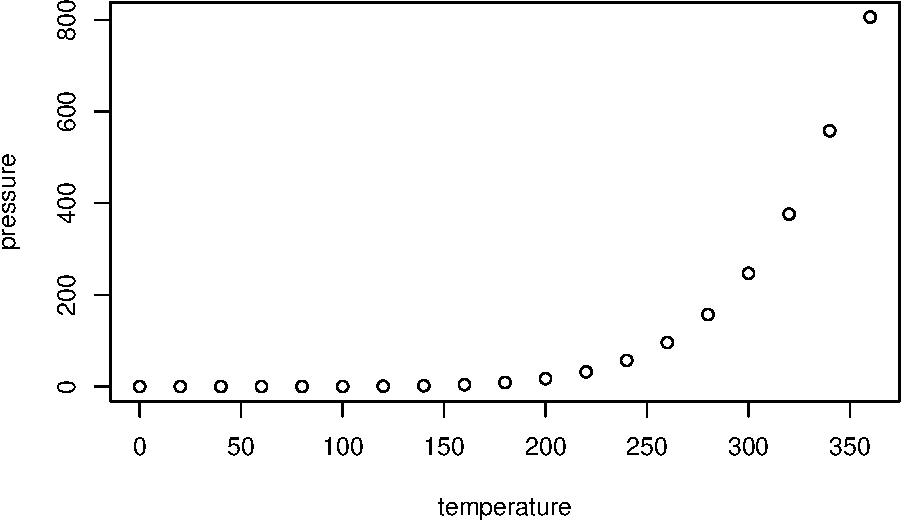
\includegraphics{4-Workshop_examples_files/figure-latex/pressure-1.pdf}
\caption{Figure of something at \(40^\circ 10^\prime\).
\label{fig:pressure}}
\end{figure}

This is inlinemath mode for Latex \(40^\circ 10^\prime\)

Note, you need extra \textbackslash{}s when using LaTeX syntax within an
R code chunk, or when inserting a backslash in R markdown. The same goes
with percent signs and any other LaTeX reserved symbol. You can use a \%
\(\%\)

\FloatBarrier

We can now reference Figure \ref{fig:pressure}. Note where this text
ends up.

Note that the \texttt{echo\ =\ FALSE} parameter was added to the code
chunk to prevent printing of the R code that generated the plot.

\section{Tables}\label{tables}

\begin{table}[ht]
\centering
\caption{This is where you write your caption} 
\label{tab:Table_example}
\scalebox{0.7}{
\begin{tabular}{rrrrrrrrrrr}
  \hline
Sample & Test1 & Test2 & Test3 & Test4 & Test5 & Test6 & Test7 & Test8 & Test9 & Test10 \\ 
  \hline
 1 & 333000000000.0 & 97.0 & 45 & 7169 & 5656 & 2642 & 8534 & 9173.0 & 230 & 2733 \\ 
   3 & 345.0 & 976.0 &  6 & 105 & 6382 & 2277 & 5848 & 7339495403.0 & 8613 & 5025 \\ 
   5 & 34.0 & 3333333333.0 &  7 & 2395 & 5632 & 5542 & 1645 & 380.0 & 1263 & 6728 \\ 
   7 & 234.0 & 34.0 & 46 & 5619 & 6063 & 8973 & 9362 & 1870.0 & 7651 & 683 \\ 
   9 & 234.0 & 0.0 & 45 & 6531 & 6824 & 3609 & 7627 & 3363.0 & 1534 & 8333 \\ 
   \hline
\end{tabular}
}
\end{table}

\begin{table}[ht]
\centering
\caption{Taiwan data} 
\label{tab:Taiwan}
\begin{tabular}{rrrrrrr}
  \hline
spp & Year & Catch\_KG & AreaSwept\_km2 & Vessel & Lat & Lon \\ 
  \hline
  1 & 1970 & 0.00 & 0.01 &   0 & 19.50 & 112.50 \\ 
    1 & 1970 & 0.00 & 0.01 &   0 & 21.50 & 116.00 \\ 
    1 & 1970 & 0.00 & 0.01 &   0 & 21.50 & 116.50 \\ 
    1 & 1970 & 0.00 & 0.01 &   0 & 23.00 & 118.00 \\ 
    1 & 1970 & 0.00 & 0.01 &   0 & 25.50 & 123.00 \\ 
    1 & 1970 & 0.00 & 0.01 &   0 & 25.50 & 123.50 \\ 
    1 & 1970 & 0.00 & 0.01 &   0 & 26.00 & 123.00 \\ 
    1 & 1970 & 0.00 & 0.01 &   0 & 26.50 & 121.00 \\ 
    1 & 1970 & 0.00 & 0.01 &   0 & 26.50 & 124.00 \\ 
    1 & 1970 & 0.00 & 0.01 &   0 & 28.00 & 122.50 \\ 
    1 & 1970 & 0.00 & 0.01 &   0 & 29.50 & 124.00 \\ 
    1 & 1970 & 0.07 & 0.01 &   0 & 22.50 & 118.00 \\ 
    1 & 1970 & 0.10 & 0.01 &   0 & 28.00 & 122.50 \\ 
    1 & 1970 & 0.50 & 0.01 &   0 & 16.50 & 109.00 \\ 
   \hline
\end{tabular}
\end{table}

Try changing the R chunk options above.

We can now reference Table \ref{tab:Table_example}.

Now, try putting the R code chunk within and HTML comment.

\section{Create you own table}\label{create-you-own-table}

Either create a .csv file or copy one into the repo folder on your
computer.

Now, create a table!

\section{Math mode}\label{math-mode}

You can use LaTeX math mode both inline and for inserting equations.
It's handy for using inline math mode for management measure and
lat/long.

Inline looks like this: \(SPR_{40\%}\)\\
*Note the \% sign has a ~when used in math mode, but not in R markdown
text.

To get degrees and minutes type: \(40^\circ 10^\prime\)

\section*{References}\label{references}
\addcontentsline{toc}{section}{References}

\hypertarget{refs}{}
\hypertarget{ref-Love2002}{}
Love, M., Yoklavich, M., and Thorsteinson, L. 2002. The rockfishes of
the northeast Pacific. University of California Press, Berkeley, CA,
USA.

\end{document}
